\chapter{Holtrop en Mennen (oud)}
\section{Weerstandsschatting met de Holtrop-Mennen methode}
\label{sec:holtrop}

De totale weerstand van het schip \emph{De Jansje} in varende conditie is geschat met behulp van de statistische regressiemethode van Holtrop en Mennen, zoals gepubliceerd in \cite{Holtrop1984}. Deze methode is geldig voor de varende conditie in zeewater ($\rho = 1025\ \mathrm{kg/m^3}$) bij $15\,^{\circ}\mathrm{C}$, zonder golven.

De totale weerstand wordt opgesplitst in de volgende componenten \cite{Holtrop1984}:

\begin{equation}
    R_\mathrm{totaal} = R_F(1+k_1) + R_{APP} + R_W + R_B + R_{TR} + R_A
    \label{eq:Rtot}
\end{equation}

\noindent waarbij:
\begin{itemize}
    \item $R_F$ de wrijvingsweerstand volgens de ITTC-1957 formulering is,
    \item $(1+k_1)$ de vormfactor van de romp is,
    \item $R_{APP}$ de aanhangselweerstand is (bijv.\ roer, schroefassen),
    \item $R_W$ de golfweerstand is,
    \item $R_B$ de extra weerstand door een boegbulb nabij het wateroppervlak is,
    \item $R_{TR}$ de drukweerstand van een geïmmergeerde spiegel is,
    \item $R_A$ de modelschaalkorrelatieallowance ($C_A$) is, inclusief de ruwheidsallowance $\Delta C_F$.
\end{itemize}

De wrijvingsweerstand wordt berekend als:
\begin{equation}
    R_F = \frac{1}{2}\,\rho\,V^2\,S\,C_F, \qquad
    C_F = \frac{0.075}{(\log Re - 2)^2}
    \label{eq:RF}
\end{equation}

De golfweerstand voor het opererende Froude-getal-gebied ($F_n \leq 0.4$) is:
\begin{equation}
    R_W = c_1\,c_2\,c_5\,\nabla\,\rho\,g \exp\!\bigl[m_1 F_n^d + m_4 \cos(\lambda F_n^{-2})\bigr]
    \label{eq:RW}
\end{equation}

\noindent De coëfficiënten $c_1, c_2, c_5, m_1, m_4, \lambda$ zijn uitdrukkingen in de scheepsparameters $L_{wl}$, $B$, $T$, $C_B$, $C_P$, $C_{wp}$, $C_M$ en $L_{CB}$. De geldigheidsrange van de methode omvat o.a.:
$0.55 \leq C_P \leq 0.85$, $3.9 \leq L/B \leq 14.9$ en $2.1 \leq B/T \leq 4.0$.

\newpage
\subsection{Scheepsgegevens}

\begin{table}[h!]
\centering
\caption{Invoerparameters Holtrop-schatting, \emph{t Jansje} (varende conditie)}
\label{tab:holtrop_input}
\begin{tabular}{llll}
\toprule
Parameter & Symbool & Waarde & Eenheid \\
\midrule
Lengte waterlijn           & $L_{wl}$  & 22.22    & m       \\
Breedte waterlijn          & $B$       & 4.36     & m       \\
Diepgang achterschip       & $T_{APP}$ & 1.50     & m       \\
Diepgang voorschip         & $T_{FPP}$ & 1.50     & m       \\
Gemiddelde diepgang        & $T_m$     & 1.50     & m       \\
Verdringingsvolume         & $\nabla$  & 73.0     & m$^3$   \\
Hoofdspantcoëfficiënt      & $C_M$     & 0.90     & --      \\
Waterplancoëfficiënt       & $C_{wp}$  & 0.795    & --      \\
Blokcoëfficiënt            & $C_B$     & 0.502    & --      \\
Prismatische coëfficiënt   & $C_P$     & 0.558    & --      \\
Halve instroomhoek         & $i_E$     & 17       & $^\circ$\\
LCB-positie (t.o.v.\ $\tfrac{1}{2}L_{wl}$) & $LCB$\% & 0.0 & \%  \\
Spiegeloppervlak           & $A_T$     & 0        & m$^2$   \\
Transversaal boegbulboppervlak & $A_{BT}$ & 0     & m$^2$   \\
Sternvormcoëfficiënt       & $C_{stern}$& 0       & --      \\
Ruwheidsmaatstaf           & $k_s$     & 150      & $\mu$m  \\
\bottomrule
\end{tabular}
\end{table}

De methode van Holtrop en Mennen is afgeleid via statistische regressie op een proefbestand van scheepsmodellen. Daardoor gelden geldigheidsranges voor de invoerparameters: buiten deze ranges kunnen de regressieformules onbetrouwbare uitkomsten geven. De spreadsheetimplementatie \cite{spreadsheet_holtrop} controleert automatisch acht geldigheidsvoorwaarden. Tabel~\ref{tab:holtrop_checks} geeft een overzicht van alle checks, de toegepaste grenswaarden, de waarde voor \emph{t Jansje} en het resultaat.

\begin{table}[h!]
\centering
\caption{Geldigheidscontroles Holtrop (1984) voor \emph{t Jansje}}
\label{tab:holtrop_checks}
\begin{tabular}{llccc}
\toprule
Parameter & Voorwaarde & Waarde \emph{t Jansje} & Geslaagd \\
\midrule
Lengte-breedte verhouding      & $3.9 \leq L_{wl}/B \leq 14.9$       & 5.10    & \cmark \\
Breedte-diepgang verhouding    & $2.1 \leq B/T \leq 4.0$             & 2.91    & \cmark \\
Prismatische coëfficiënt       & $0.55 \leq C_P \leq 0.85$           & 0.558   & \cmark \\
LCB-positie                    & $-5\% \leq LCB\% \leq +5\%$        & 0.0\%   & \cmark \\
Halve instroomhoek             & $1^\circ \leq i_E \leq 90^\circ$   & $17^\circ$ & \cmark \\
Hoogte boegbulb boven kiel     & $0 \leq h_B \leq 0.6\,T_{FPP}$     & 0       & \cmark \\
Golfweerstandsparameter        & $0.01 \leq \lambda \leq 1.07$       & 0.654   & \cmark \\
Froude-getal (bij 8~kn)        & $F_n \leq 0.77$                     & 0.279   & \cmark \\
Froude-getal (bij $>$16~kn)    & $F_n \leq 0.77$                     & $>$0.77 & $\times$   \\
\bottomrule
\end{tabular}
\end{table}

De fysische betekenis van elke check is als volgt:

\begin{itemize}
    \item \textbf{$L_{wl}/B = 5.10$} --- de lengte-breedte verhouding bepaalt de slankheidsvorm van het schip. De ondergrens (3.9) sluit brede, pontoonachtige rompen uit. De bovengrens (14.9) sluit slanke torpedo-achtige rompen uit. \emph{Jansje} valt ruim binnen het normale bereik van binnenvaartschepen.

    \item \textbf{$B/T = 2.91$} --- de breedte-diepgang verhouding bepaalt de dwarsdoorsnede-verhouding. Een waarde buiten $[2.1,\,4.0]$ zou duiden op een zeer diepgeladen ($B/T < 2.1$) of extreem ondiepstekend schip ($B/T > 4.0$). \emph{t Jansje} heeft een evenwichtige dwarsvorm met $B/T = 2.91$.

    \item \textbf{$C_P = 0.558$} --- de prismatische coëfficiënt beschrijft hoe vol de romp is vergeleken met een cilinder met het grootste spant als doorsnede. De ondergrens van 0.55 sluit zeer slanke jachten en snelvarende schepen uit, voor wie de regressie niet is gecalibreerd. \emph{t Jansje} zit net boven de grens ($C_P = 0.558$), wat passend is voor een langzaamvarend vrachtschip.

    \item \textbf{$LCB\% = 0.0\%$} --- de longitudinale positie van het drijfpunt (gemeten in procenten van $L_{wl}$ ten opzichte van het midden van het schip) heeft een grote impact op de weerstandsformules. De range $[-5\%,\,+5\%]$ dekt vrijwel alle conventionele scheepsvormen. Een waarde van 0\% betekent dat het drijfpunt precies op het midden ligt.

    \item \textbf{$i_E = 17^\circ$} --- de halve instroomhoek van de waterlijn aan de boeg beïnvloedt de golfweerstand via coëfficiënt $c_1$. Waarden buiten $[1^\circ,\,90^\circ]$ zijn geometrisch niet zinvol of niet geregresseerd. Een waarde van $17^\circ$ past bij een beurtvaarder met een matig scherpe boegvorm.

    \item \textbf{$h_B = 0$} --- de hoogte van de boegbulb boven de kiel mag niet meer bedragen dan $0.6\,T_{FPP}$. Aangezien \emph{t Jansje} geen boegbulb heeft ($A_{BT} = 0$, $h_B = 0$), is deze check automatisch voldaan.

    \item \textbf{$\lambda = 0.654$} --- de interne golfweerstandsparameter $\lambda$ ($= 1.446\,C_P - 0.03\,L/B$ voor $L/B < 12$) bepaalt de golflengte-afhankelijkheid in de cosinus-term van vergelijking~\eqref{eq:RW}. De range $[0.01,\,1.07]$ garandeert dat de cosinus-term fysisch zinvolle waarden geeft. \emph{t Jansje} scoort $\lambda = 0.654$, ruim binnen de geldige range.

    \item \textbf{$F_n \leq 0.77$} --- het Froude-getal is de belangrijkste geldigheidsgrens. Boven $F_n = 0.77$ treedt planning op; de Holtrop-formules zijn uitsluitend gevalideerd voor verdringingsvaart. Bij de ontwerpsnelheid van 8~knoop geldt $F_n = 0.279$, ruimschoots binnen het geldige bereik. Pas bij snelheden boven $\approx 16$~knoop wordt $F_n > 0.77$; die snelheden zijn voor \emph{t Jansje} niet relevant.
\end{itemize}

\subsection{Afgeleide grootheden}

De methode berekent intern een aantal grootheden die direct voortvloeien uit de invoerparameters:

\begin{table}[h!]
\centering
\caption{Berekende grootheden op basis van de scheepsgeometrische invoer}
\label{tab:holtrop_derived}
\begin{tabular}{llll}
\toprule
Grootheid & Symbool & Waarde & Eenheid \\
\midrule
Vormfactor            & $(1+k_1)$    & 1.2081                & --      \\
Nat oppervlak         & $S$          & 108.82                & m$^2$   \\
Looplengte            & $L_R$        & 9.82                  & m       \\
Correlatie-allowance  & $C_A$        & $7.31 \times 10^{-4}$ & --      \\
Ruwheidsallowance     & $\Delta C_F$ & $4.31 \times 10^{-8}$ & --      \\
\bottomrule
\end{tabular}
\end{table}

De vormfactor $(1+k_1) = 1.208$ geeft aan dat de viskeuze weerstand van de romp ruim 20\% hoger is dan de vlakke plaatswrijving alleen, wat kenmerkend is voor een relatief vol maar kort schip met $C_B \approx 0.50$.

\newpage
\subsection{Resultaten}

\subsubsection{Weerstandscomponenten bij de ontwerpsnelheid}

Bij de ontwerpsnelheid van 8~knoop ($V = 4.116\ \mathrm{m/s}$, $F_n = 0.279$) resulteert de berekening in:

\begin{table}[h!]
\centering
\caption{Weerstandscomponenten bij $V = 8\ \mathrm{kn}$}
\label{tab:holtrop_results_8kn}
\begin{tabular}{lrr}
\toprule
Component & Waarde [kN] & Aandeel [\%] \\
\midrule
Wrijvingsweerstand (incl.\ vormfactor) $R_F(1+k_1)$ & 2.472 & 55.7 \\
Golfweerstand $R_W$                                  & 1.276 & 28.8 \\
Correlatie-allowance $R_A$                           & 0.691 & 15.6 \\
Aanhangselweerstand $R_{APP}$                        & 0     & 0.0  \\
Spiegelweerstand $R_{TR}$                            & 0     & 0.0  \\
Boegbulbweerstand $R_B$                              & 0     & 0.0  \\
\midrule
\textbf{Totale weerstand} $R_{totaal}$               & \textbf{4.439} & \textbf{100.0} \\
\midrule
Effectief vermogen EHP & \multicolumn{2}{c}{$18.3\ \mathrm{kW}$} \\
\bottomrule
\end{tabular}
\end{table}

De wrijvingsweerstand vormt het grootste component (55.7\%). Dit is in lijn met de verwachtingen voor een relatief langzaam binnenvaartschip met een laag Froudegetal. Bij een snelheid van 8~knopen is de golfweerstand met 28.8\% echter niet langer verwaarloosbaar. De weerstand van de aanhangsels ($R_{APP}$) is in dit model buiten beschouwing gelaten ($R_{APP} = 0$), aangezien er geen specifieke appendages zijn gemodelleerd. Dit betreft een simplificatie van de werkelijkheid; in de praktijk zal $R_{APP} > 0$, waardoor de daadwerkelijke scheepsweerstand hoger zal uitvallen.

\subsubsection{\textbf{Snelheidsreeks}}

\begin{table}[h!]
\centering
\caption{Weerstand en effectief vermogen als functie van de snelheid}
\label{tab:holtrop_speed_series}
\begin{tabular}{rrrrrrrr}
\toprule
$V$ [kn] & $V$ [m/s] & $F_n$ [-] & $R_F$ [kN] & $R_W$ [kN] & $R_A$ [kN] & $R_{tot}$ [kN] & EHP [kW] \\
\midrule
5  & 2.572 & 0.174 & 1.036 & 0.020 & 0.270 & 1.326 &  3.41 \\
6  & 3.087 & 0.209 & 1.452 & 0.123 & 0.388 & 1.963 &  6.06 \\
7  & 3.601 & 0.244 & 1.931 & 0.455 & 0.529 & 2.914 & 10.49 \\
\rowcolor{green!15}
8  & 4.116 & 0.279 & 2.472 & 1.276 & 0.691 & 4.439 & 18.27 \\
9  & 4.630 & 0.314 & 3.075 & 2.351 & 0.874 & 6.300 & 29.17 \\
10 & 5.144 & 0.348 & 3.739 & 4.397 & 1.079 & 9.215 & 47.41 \\
\bottomrule
\end{tabular}
\end{table}


\newpage
\subsection{Figuren}
\label{subsec:holtrop_figuren}

De resultaten van de Holtropschatting zijn weergegeven in vier figuren. Figuur~\ref{fig:holtrop_rtot} toont de totale weerstand als functie van de snelheid. Figuur~\ref{fig:holtrop_stacked} geeft de opbouw van de weerstand in drie componenten. Figuur~\ref{fig:holtrop_ehp} toont het effectief vermogen met markering van de ontwerpsnelheid. Figuur~\ref{fig:holtrop_pie} geeft de procentuele verdeling van de weerstandscomponenten bij 8~knoop.

% ------------------------------------------------------------------
% Figuur 1: Totale weerstand vs. snelheid
% ------------------------------------------------------------------
\begin{figure}[H]
\centering
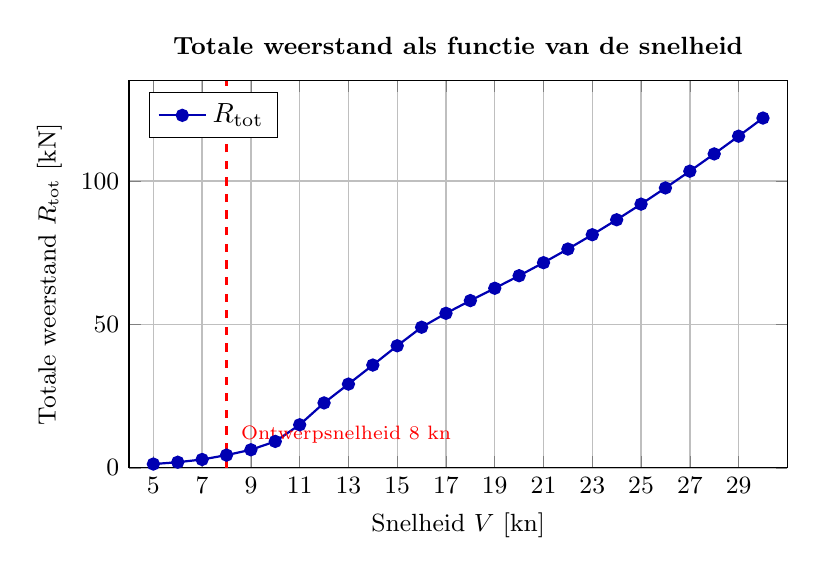
\begin{tikzpicture}
\begin{axis}[
    width  = 0.82\textwidth,
    height = 6.5cm,
    xlabel = {Snelheid $V$ [kn]},
    ylabel = {Totale weerstand $R_\mathrm{tot}$ [kN]},
    title  = {Totale weerstand als functie van de snelheid},
    xmin=4, xmax=31,
    ymin=0, ymax=135,
    xtick={5,7,9,11,13,15,17,19,21,23,25,27,29},
    grid=both,
    grid style={line width=0.3pt, draw=gray!30},
    major grid style={line width=0.5pt, draw=gray!50},
    legend pos=north west,
    tick label style={font=\small},
    label style={font=\small},
    title style={font=\small\bfseries},
]
\addplot[
    color=blue!70!black, thick, mark=*, mark size=2pt,
] coordinates {
    (5,1.3265)(6,1.9634)(7,2.9142)(8,4.4391)(9,6.2999)(10,9.2149)
    (11,15.0227)(12,22.6354)(13,29.1946)(14,35.8332)(15,42.5505)
    (16,49.0182)(17,53.8739)(18,58.2992)(19,62.6043)(20,66.9766)
    (21,71.5172)(22,76.2736)(23,81.2624)(24,86.4828)(25,91.9253)
    (26,97.5756)(27,103.4179)(28,109.4359)(29,115.6139)(30,121.9369)
};
\addlegendentry{$R_\mathrm{tot}$}
\addplot[red, dashed, thick, forget plot]
    coordinates {(8,0)(8,135)};
\node[red, font=\scriptsize, anchor=south west] at (axis cs:8.2,5)
    {Ontwerpsnelheid 8~kn};
\end{axis}
\end{tikzpicture}
\caption{Totale weerstand van \emph{t Jansje} als functie van de snelheid,
         berekend met de methode van Holtrop~\cite{Holtrop1984}.
         De sterke toename boven 10~knoop is kenmerkend voor het
         golfweerstandshump bij $F_n \approx 0.30$--$0.35$.}
\label{fig:holtrop_rtot}
\end{figure}

% ------------------------------------------------------------------
% Figuur 2: Gestapelde weerstandscomponenten (5-14 kn)
% FIX: named paths worden eerst gedeclareerd, fill between daarna
% ------------------------------------------------------------------
\begin{figure}[H]
\centering
\begin{tikzpicture}
\begin{axis}[
    width  = 0.82\textwidth,
    height = 6.5cm,
    xlabel = {Snelheid $V$ [kn]},
    ylabel = {Weerstand [kN]},
    title  = {Weerstandscomponenten (gestapeld, 5--14~kn)},
    xmin=4.5, xmax=14.5,
    ymin=0, ymax=40,
    xtick={5,6,7,8,9,10,11,12,13,14},
    grid=both,
    grid style={line width=0.3pt, draw=gray!30},
    major grid style={line width=0.5pt, draw=gray!50},
    legend pos=north west,
    legend style={font=\small},
    tick label style={font=\small},
    label style={font=\small},
    title style={font=\small\bfseries},
]
% Stap 1: definieer alle named paths EERST
\addplot[name path=zero, draw=none, forget plot]
    coordinates {(5,0)(6,0)(7,0)(8,0)(9,0)(10,0)(11,0)(12,0)(13,0)(14,0)};

\addplot[name path=RF, draw=none, forget plot] coordinates {
    (5,1.0363)(6,1.4516)(7,1.9306)(8,2.4722)(9,3.0751)
    (10,3.7386)(11,4.4617)(12,5.2438)(13,6.0842)(14,6.9823)
};
\addplot[name path=RFRW, draw=none, forget plot] coordinates {
    (5,1.0567)(6,1.5749)(7,2.3855)(8,3.7485)(9,5.4259)
    (10,8.1359)(11,13.7170)(12,21.0815)(13,27.3710)(14,33.7182)
};
\addplot[name path=RFRWRA, draw=none, forget plot] coordinates {
    (5,1.3264)(6,1.9634)(7,2.9142)(8,4.4391)(9,6.2999)
    (10,9.2149)(11,15.0227)(12,22.6353)(13,29.1946)(14,35.8332)
};

% Stap 2: fill between op de gedeclareerde paths
\addplot[fill=blue!40, fill opacity=0.75, draw=none, area legend]
    fill between[of=RF and zero];
\addlegendentry{$R_F(1{+}k_1)$}

\addplot[fill=red!45, fill opacity=0.75, draw=none, area legend]
    fill between[of=RFRW and RF];
\addlegendentry{$R_W$}

\addplot[fill=yellow!60, fill opacity=0.85, draw=none, area legend]
    fill between[of=RFRWRA and RFRW];
\addlegendentry{$R_A$}

% Stap 3: zichtbare lijnen bovenop
\addplot[blue!70!black, thick, mark=*, mark size=1.8pt, forget plot] coordinates {
    (5,1.0363)(6,1.4516)(7,1.9306)(8,2.4722)(9,3.0751)
    (10,3.7386)(11,4.4617)(12,5.2438)(13,6.0842)(14,6.9823)
};
\addplot[red!60!black, thick, forget plot] coordinates {
    (5,1.0567)(6,1.5749)(7,2.3855)(8,3.7485)(9,5.4259)
    (10,8.1359)(11,13.7170)(12,21.0815)(13,27.3710)(14,33.7182)
};
\addplot[yellow!60!black, thick, forget plot] coordinates {
    (5,1.3264)(6,1.9634)(7,2.9142)(8,4.4391)(9,6.2999)
    (10,9.2149)(11,15.0227)(12,22.6353)(13,29.1946)(14,35.8332)
};
\addplot[red, dashed, thick, forget plot]
    coordinates {(8,0)(8,40)};
\end{axis}
\end{tikzpicture}
\caption{Gestapelde weerstandscomponenten voor \emph{t Jansje} in het bereik
         5--14~knoop. $R_W$ neemt snel toe boven 7~knoop,
         terwijl $R_F$ bij lage snelheden het grootste aandeel heeft.}
\label{fig:holtrop_stacked}
\end{figure}

% ------------------------------------------------------------------
% Figuur 3: EHP vs. snelheid
% ------------------------------------------------------------------
\begin{figure}[H]
\centering
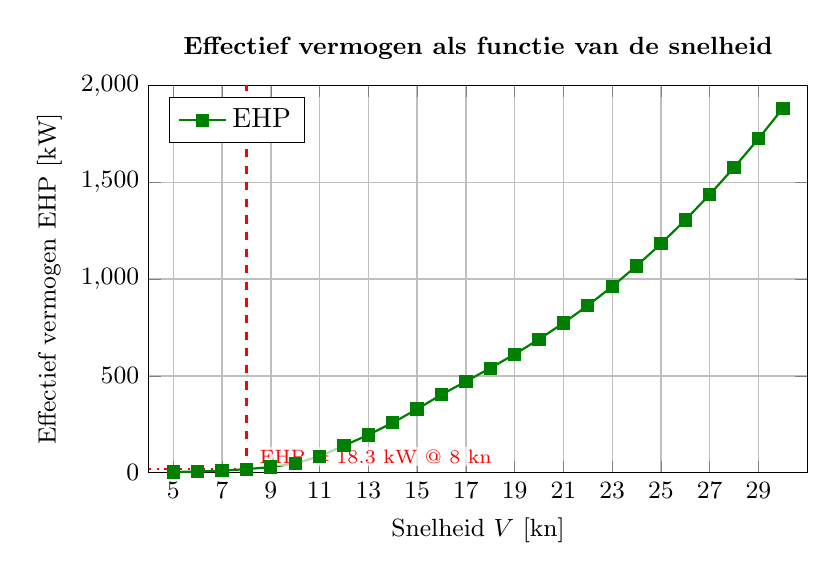
\begin{tikzpicture}
\begin{axis}[
    width  = 0.82\textwidth,
    height = 6.5cm,
    xlabel = {Snelheid $V$ [kn]},
    ylabel = {Effectief vermogen EHP [kW]},
    title  = {Effectief vermogen als functie van de snelheid},
    xmin=4, xmax=31,
    ymin=0, ymax=2000,
    xtick={5,7,9,11,13,15,17,19,21,23,25,27,29},
    grid=both,
    grid style={line width=0.3pt, draw=gray!30},
    major grid style={line width=0.5pt, draw=gray!50},
    legend pos=north west,
    tick label style={font=\small},
    label style={font=\small},
    title style={font=\small\bfseries},
]
\addplot[
    color=green!50!black, thick, mark=square*, mark size=2pt,
] coordinates {
    (5,3.412)(6,6.060)(7,10.494)(8,18.269)(9,29.169)(10,47.406)
    (11,85.012)(12,139.736)(13,195.247)(14,258.078)(15,328.348)
    (16,403.474)(17,471.157)(18,539.850)(19,611.922)(20,689.114)
    (21,772.623)(22,863.247)(23,961.514)(24,1067.773)(25,1182.260)
    (26,1305.127)(27,1436.473)(28,1576.362)(29,1724.829)(30,1881.891)
};
\addlegendentry{EHP}
\addplot[red, dashed, thick, forget plot]
    coordinates {(8,0)(8,2000)};
\addplot[red, dotted, thick, forget plot]
    coordinates {(4,18.269)(8,18.269)};
\node[red, font=\scriptsize, anchor=south west,
      fill=white, fill opacity=0.7, text opacity=1,
      inner sep=1pt] at (axis cs:8.4,30)
    {EHP $= 18.3$~kW @ 8~kn};
\end{axis}
\end{tikzpicture}
\caption{Effectief vermogen van \emph{Jansje} als functie van de snelheid. Bij de ontwerpsnelheid van 8~knoop is het effectief vermogen $\mathrm{EHP} = 18.3\ \mathrm{kW}$. Het daadwerkelijk te installeren vermogen ligt hoger. Dit komt doordat we nog moeten compenseren voor verliezen in de aandrijflijn ($\eta_D$) en we operationele marges moeten aanhouden.}
\label{fig:holtrop_ehp}
\end{figure}

% ------------------------------------------------------------------
% Figuur 4: Taartdiagram (puur TikZ, geen \matrix)
% FIX: \matrix vervangen door handmatige legenda met \node
% ------------------------------------------------------------------
\begin{figure}[H]
\centering
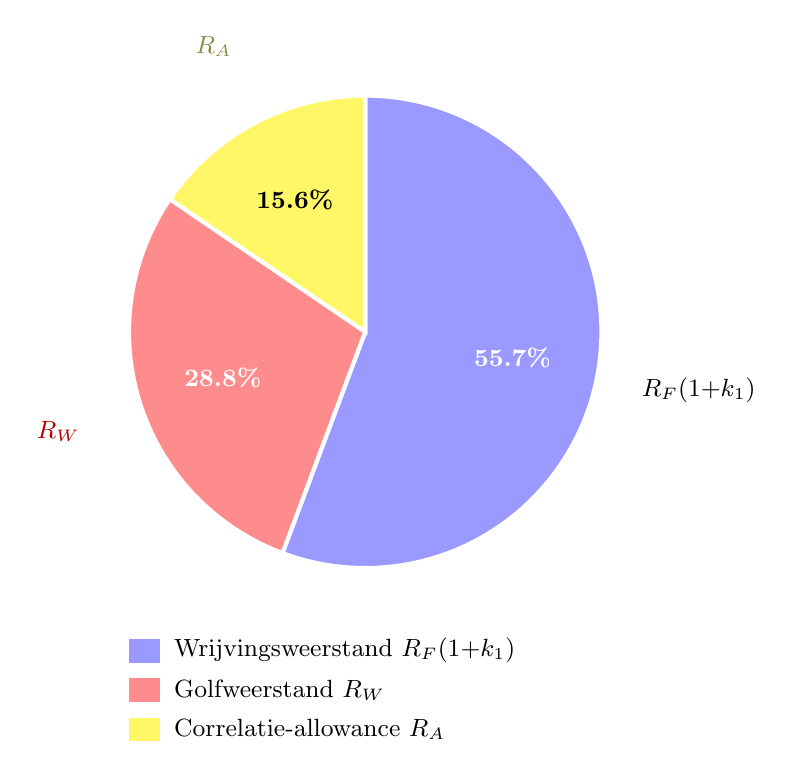
\begin{tikzpicture}
\def\R{3.0cm}

% Segment 1: R_F (55.7%) van 90 tot -110.5 graden
\fill[blue!40, draw=white, line width=1.5pt]
    (0,0) -- ({cos(90)*\R},{sin(90)*\R})
    arc[start angle=90, end angle=-110.5, radius=\R] -- cycle;

% Segment 2: R_W (28.8%) van -110.5 tot -214.2 graden
\fill[red!45, draw=white, line width=1.5pt]
    (0,0) -- ({cos(-110.5)*\R},{sin(-110.5)*\R})
    arc[start angle=-110.5, end angle=-214.2, radius=\R] -- cycle;

% Segment 3: R_A (15.5%) van -214.2 tot -270 graden
\fill[yellow!60, draw=white, line width=1.5pt]
    (0,0) -- ({cos(-214.2)*\R},{sin(-214.2)*\R})
    arc[start angle=-214.2, end angle=-270, radius=\R] -- cycle;

% Percentages in de segmenten
\node[font=\small\bfseries, white] at ({cos(-10)*1.9cm},{sin(-10)*1.9cm})
    {55.7\%};
\node[font=\small\bfseries, white] at ({cos(-162)*1.9cm},{sin(-162)*1.9cm})
    {28.8\%};
\node[font=\small\bfseries] at ({cos(-242)*1.9cm},{sin(-242)*1.9cm})
    {15.6\%};

% Labels buiten de taart
\node[font=\small\bfseries, align=left] at ({cos(-10)*(\R+1.3cm)},{sin(-10)*(\R+1.3cm)})
    {$R_F(1{+}k_1)$};
\node[font=\small\bfseries, text=red!70!black, align=right]
    at ({cos(-162)*(\R+1.1cm)},{sin(-162)*(\R+1.1cm)}) {$R_W$};
\node[font=\small\bfseries, text=yellow!50!black, align=left]
    at ({cos(-242)*(\R+1.1cm)},{sin(-242)*(\R+1.1cm)}) {$R_A$};

% Handmatige legenda onder de taart (geen \matrix)
\fill[blue!40]  (-3.0,-4.2) rectangle (-2.6,-3.9);
\node[right, font=\small] at (-2.55,-4.05) {Wrijvingsweerstand $R_F(1{+}k_1)$};

\fill[red!45]   (-3.0,-4.7) rectangle (-2.6,-4.4);
\node[right, font=\small] at (-2.55,-4.55) {Golfweerstand $R_W$};

\fill[yellow!60](-3.0,-5.2) rectangle (-2.6,-4.9);
\node[right, font=\small] at (-2.55,-5.05) {Correlatie-allowance $R_A$};
\end{tikzpicture}
\caption{Procentuele verdeling van de weerstandscomponenten bij de
         ontwerpsnelheid van 8~knoop ($R_\mathrm{tot} = 4.44\ \mathrm{kN}$).
         De wrijvingsweerstand is dominant (55.7\%), terwijl de golfweerstand
         met 28.8\% al significant is bij $F_n = 0.279$.}
\label{fig:holtrop_pie}
\end{figure}
\newpage
\subsection{Validatie en beperkingen}

De methode van Holtrop en Mennen is wereldwijd de meest gebruikte statistische methode voor vroege ontwerpfasen. De geschatte nauwkeurigheid bedraagt doorgaans $\pm 5$--$10\%$ voor de totale weerstand, mits de scheepsparameters binnen de geldigheidsrange vallen \cite{Holtrop1984, Molland2011}.

Voor \emph{t Jansje} gelden de volgende kanttekeningen:

\begin{itemize}
    \item \textbf{Aanhangsels}: Geen roer, schroefas of kielplaat ingevoerd ($R_{APP} = 0$). Bij implementatie van een definitief aandrijfconcept dient $R_{APP}$ nader bepaald te worden.
    \item \textbf{Ondiepwater-effect}: De methode is ontwikkeld voor diepwater. Het vaargebied (Nieuwe Maas, Maassluis) kan ondiepwater-effecten hebben die de weerstand verhogen.
    \item \textbf{Golven en wind}: De berekening is geldig voor kalm water. Operationele marges voor golfweerstand ($R_{AW}$) en windweerstand ($R_{AA}$) zijn niet meegenomen.
\end{itemize}

Ondanks deze beperkingen geeft de Holtrop-schatting een betrouwbare ondergrens voor het benodigde aandrijfvermogen en is daarmee geschikt als uitgangspunt voor de vergelijking van alternatieve aandrijfconcepten.

\subsection*{Conclusie}

Bij de ontwerpsnelheid van 8~knoop bedraagt de totale weerstand van \emph{t Jansje} $R_{tot} = 4.44\ \mathrm{kN}$, overeenkomend met een effectief vermogen van $\mathrm{EHP} = 18.3\ \mathrm{kW}$. Het benodigde geïnstalleerde vermogen zal hoger uitvallen nadat rendementsverlies van de aandrijflijn ($\eta_D$).